\documentclass[tikz,border=2pt]{standalone}
\usepackage{tikz}
\usetikzlibrary{arrows.meta,positioning,fit,shapes.geometric}
\begin{document}
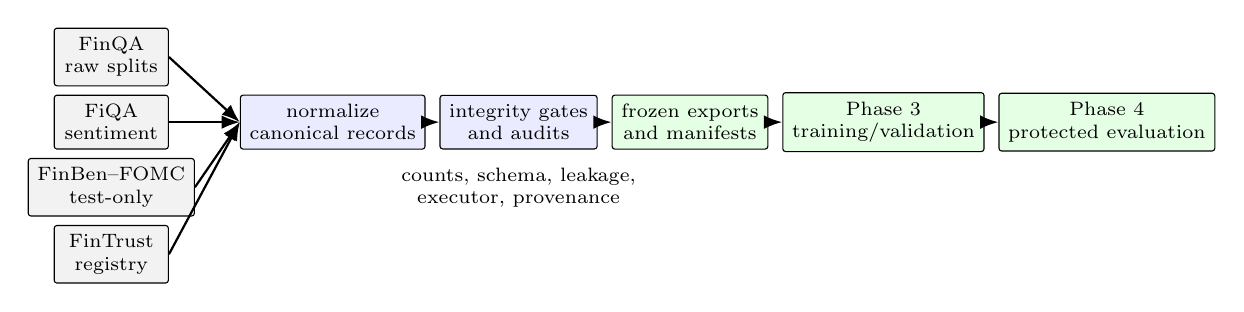
\begin{tikzpicture}[node distance=3pt and 5pt, >=Latex,
  source/.style={draw, rounded corners=1pt, fill=gray!10, align=center,
    minimum width=1.45cm, minimum height=0.62cm, font=\scriptsize},
  gate/.style={draw, rounded corners=1pt, fill=blue!8, align=center,
    minimum width=1.55cm, minimum height=0.62cm, font=\scriptsize},
  output/.style={draw, rounded corners=1pt, fill=green!10, align=center,
    minimum width=1.55cm, minimum height=0.62cm, font=\scriptsize},
  arrow/.style={->, thick}]
\node[source] (finqa) {FinQA\\raw splits};
\node[source, below=of finqa] (fiqa) {FiQA\\sentiment};
\node[source, below=of fiqa] (fomc) {FinBen--FOMC\\test-only};
\node[source, below=of fomc] (trust) {FinTrust\\registry};
\node[gate, right=9mm of fiqa] (normalize) {normalize\\canonical records};
\node[gate, right=of normalize] (checks) {integrity gates\\and audits};
\node[output, right=of checks] (exports) {frozen exports\\and manifests};
\node[output, right=of exports] (p3) {Phase 3\\training/validation};
\node[output, right=of p3] (p4) {Phase 4\\protected evaluation};
\draw[arrow] (finqa.east) -- (normalize.west);
\draw[arrow] (fiqa.east) -- (normalize.west);
\draw[arrow] (fomc.east) -- (normalize.west);
\draw[arrow] (trust.east) -- (normalize.west);
\draw[arrow] (normalize) -- (checks);
\draw[arrow] (checks) -- (exports);
\draw[arrow] (exports) -- (p3);
\draw[arrow] (p3) -- (p4);
\node[below=3pt of checks, align=center, font=\scriptsize] {counts, schema, leakage,\\executor, provenance};
\end{tikzpicture}
\end{document}
